% Options for packages loaded elsewhere
\PassOptionsToPackage{unicode}{hyperref}
\PassOptionsToPackage{hyphens}{url}
\PassOptionsToPackage{dvipsnames,svgnames*,x11names*}{xcolor}
%
\documentclass[
  ignorenonframetext,
]{beamer}
\usepackage{pgfpages}
\setbeamertemplate{caption}[numbered]
\setbeamertemplate{caption label separator}{: }
\setbeamercolor{caption name}{fg=normal text.fg}
\beamertemplatenavigationsymbolsempty
% Prevent slide breaks in the middle of a paragraph
\widowpenalties 1 10000
\raggedbottom
\setbeamertemplate{part page}{
  \centering
  \begin{beamercolorbox}[sep=16pt,center]{part title}
    \usebeamerfont{part title}\insertpart\par
  \end{beamercolorbox}
}
\setbeamertemplate{section page}{
  \centering
  \begin{beamercolorbox}[sep=12pt,center]{part title}
    \usebeamerfont{section title}\insertsection\par
  \end{beamercolorbox}
}
\setbeamertemplate{subsection page}{
  \centering
  \begin{beamercolorbox}[sep=8pt,center]{part title}
    \usebeamerfont{subsection title}\insertsubsection\par
  \end{beamercolorbox}
}
\AtBeginPart{
  \frame{\partpage}
}
\AtBeginSection{
  \ifbibliography
  \else
    \frame{\sectionpage}
  \fi
}
\AtBeginSubsection{
  \frame{\subsectionpage}
}
\usepackage{lmodern}
\usepackage{amssymb,amsmath}
\usepackage{ifxetex,ifluatex}
\ifnum 0\ifxetex 1\fi\ifluatex 1\fi=0 % if pdftex
  \usepackage[T1]{fontenc}
  \usepackage[utf8]{inputenc}
  \usepackage{textcomp} % provide euro and other symbols
\else % if luatex or xetex
  \usepackage{unicode-math}
  \defaultfontfeatures{Scale=MatchLowercase}
  \defaultfontfeatures[\rmfamily]{Ligatures=TeX,Scale=1}
\fi
\usetheme[]{AnnArbor}
\usecolortheme{dove}
% Use upquote if available, for straight quotes in verbatim environments
\IfFileExists{upquote.sty}{\usepackage{upquote}}{}
\IfFileExists{microtype.sty}{% use microtype if available
  \usepackage[]{microtype}
  \UseMicrotypeSet[protrusion]{basicmath} % disable protrusion for tt fonts
}{}
\makeatletter
\@ifundefined{KOMAClassName}{% if non-KOMA class
  \IfFileExists{parskip.sty}{%
    \usepackage{parskip}
  }{% else
    \setlength{\parindent}{0pt}
    \setlength{\parskip}{6pt plus 2pt minus 1pt}}
}{% if KOMA class
  \KOMAoptions{parskip=half}}
\makeatother
\usepackage{xcolor}
\IfFileExists{xurl.sty}{\usepackage{xurl}}{} % add URL line breaks if available
\IfFileExists{bookmark.sty}{\usepackage{bookmark}}{\usepackage{hyperref}}
\hypersetup{
  pdftitle={Statistical Inference: the sign test},
  colorlinks=true,
  linkcolor=Maroon,
  filecolor=Maroon,
  citecolor=Blue,
  urlcolor=blue,
  pdfcreator={LaTeX via pandoc}}
\urlstyle{same} % disable monospaced font for URLs
\newif\ifbibliography
\usepackage{color}
\usepackage{fancyvrb}
\newcommand{\VerbBar}{|}
\newcommand{\VERB}{\Verb[commandchars=\\\{\}]}
\DefineVerbatimEnvironment{Highlighting}{Verbatim}{commandchars=\\\{\}}
% Add ',fontsize=\small' for more characters per line
\usepackage{framed}
\definecolor{shadecolor}{RGB}{248,248,248}
\newenvironment{Shaded}{\begin{snugshade}}{\end{snugshade}}
\newcommand{\AlertTok}[1]{\textcolor[rgb]{0.94,0.16,0.16}{#1}}
\newcommand{\AnnotationTok}[1]{\textcolor[rgb]{0.56,0.35,0.01}{\textbf{\textit{#1}}}}
\newcommand{\AttributeTok}[1]{\textcolor[rgb]{0.77,0.63,0.00}{#1}}
\newcommand{\BaseNTok}[1]{\textcolor[rgb]{0.00,0.00,0.81}{#1}}
\newcommand{\BuiltInTok}[1]{#1}
\newcommand{\CharTok}[1]{\textcolor[rgb]{0.31,0.60,0.02}{#1}}
\newcommand{\CommentTok}[1]{\textcolor[rgb]{0.56,0.35,0.01}{\textit{#1}}}
\newcommand{\CommentVarTok}[1]{\textcolor[rgb]{0.56,0.35,0.01}{\textbf{\textit{#1}}}}
\newcommand{\ConstantTok}[1]{\textcolor[rgb]{0.00,0.00,0.00}{#1}}
\newcommand{\ControlFlowTok}[1]{\textcolor[rgb]{0.13,0.29,0.53}{\textbf{#1}}}
\newcommand{\DataTypeTok}[1]{\textcolor[rgb]{0.13,0.29,0.53}{#1}}
\newcommand{\DecValTok}[1]{\textcolor[rgb]{0.00,0.00,0.81}{#1}}
\newcommand{\DocumentationTok}[1]{\textcolor[rgb]{0.56,0.35,0.01}{\textbf{\textit{#1}}}}
\newcommand{\ErrorTok}[1]{\textcolor[rgb]{0.64,0.00,0.00}{\textbf{#1}}}
\newcommand{\ExtensionTok}[1]{#1}
\newcommand{\FloatTok}[1]{\textcolor[rgb]{0.00,0.00,0.81}{#1}}
\newcommand{\FunctionTok}[1]{\textcolor[rgb]{0.00,0.00,0.00}{#1}}
\newcommand{\ImportTok}[1]{#1}
\newcommand{\InformationTok}[1]{\textcolor[rgb]{0.56,0.35,0.01}{\textbf{\textit{#1}}}}
\newcommand{\KeywordTok}[1]{\textcolor[rgb]{0.13,0.29,0.53}{\textbf{#1}}}
\newcommand{\NormalTok}[1]{#1}
\newcommand{\OperatorTok}[1]{\textcolor[rgb]{0.81,0.36,0.00}{\textbf{#1}}}
\newcommand{\OtherTok}[1]{\textcolor[rgb]{0.56,0.35,0.01}{#1}}
\newcommand{\PreprocessorTok}[1]{\textcolor[rgb]{0.56,0.35,0.01}{\textit{#1}}}
\newcommand{\RegionMarkerTok}[1]{#1}
\newcommand{\SpecialCharTok}[1]{\textcolor[rgb]{0.00,0.00,0.00}{#1}}
\newcommand{\SpecialStringTok}[1]{\textcolor[rgb]{0.31,0.60,0.02}{#1}}
\newcommand{\StringTok}[1]{\textcolor[rgb]{0.31,0.60,0.02}{#1}}
\newcommand{\VariableTok}[1]{\textcolor[rgb]{0.00,0.00,0.00}{#1}}
\newcommand{\VerbatimStringTok}[1]{\textcolor[rgb]{0.31,0.60,0.02}{#1}}
\newcommand{\WarningTok}[1]{\textcolor[rgb]{0.56,0.35,0.01}{\textbf{\textit{#1}}}}
\usepackage{longtable,booktabs}
\usepackage{caption}
% Make caption package work with longtable
\makeatletter
\def\fnum@table{\tablename~\thetable}
\makeatother
\usepackage{graphicx}
\makeatletter
\def\maxwidth{\ifdim\Gin@nat@width>\linewidth\linewidth\else\Gin@nat@width\fi}
\def\maxheight{\ifdim\Gin@nat@height>\textheight\textheight\else\Gin@nat@height\fi}
\makeatother
% Scale images if necessary, so that they will not overflow the page
% margins by default, and it is still possible to overwrite the defaults
% using explicit options in \includegraphics[width, height, ...]{}
\setkeys{Gin}{width=\maxwidth,height=\maxheight,keepaspectratio}
% Set default figure placement to htbp
\makeatletter
\def\fps@figure{htbp}
\makeatother
\setlength{\emergencystretch}{3em} % prevent overfull lines
\providecommand{\tightlist}{%
  \setlength{\itemsep}{0pt}\setlength{\parskip}{0pt}}
\setcounter{secnumdepth}{-\maxdimen} % remove section numbering
\usepackage{multicol}

\title{Statistical Inference: the sign test}
\author{}
\date{\vspace{-2.5em}}

\begin{document}
\frame{\titlepage}

\begin{frame}[fragile]
knitr::opts\_chunk\(set(fig.height = 5) # knitr::opts_chunk\)set(echo =
FALSE) options(width=52) knitr::opts\_chunk\$set(dev = `pdf')

\begin{verbatim}







## Duality between confidence intervals and hypothesis tests 
- Tests and CIs really do the same thing, if you look at them the right
way. They are both telling you something about a parameter, and
they use same things about data.
- To illustrate, some data (two groups):

```r
my_url <- "http://www.utsc.utoronto.ca/~butler/c32/duality.txt"
twogroups <- read_delim(my_url," ")
\end{verbatim}

\begin{verbatim}
## 
## -- Column specification --------------------------------------------------------
## cols(
##   y = col_double(),
##   group = col_double()
## )
\end{verbatim}
\end{frame}

\begin{frame}[fragile]{The data}
\protect\hypertarget{the-data}{}
\footnotesize

\begin{Shaded}
\begin{Highlighting}[]
\NormalTok{twogroups}
\end{Highlighting}
\end{Shaded}

\begin{longtable}[]{@{}rr@{}}
\toprule
y & group\tabularnewline
\midrule
\endhead
10 & 1\tabularnewline
11 & 1\tabularnewline
11 & 1\tabularnewline
13 & 1\tabularnewline
13 & 1\tabularnewline
14 & 1\tabularnewline
14 & 1\tabularnewline
15 & 1\tabularnewline
16 & 1\tabularnewline
13 & 2\tabularnewline
13 & 2\tabularnewline
14 & 2\tabularnewline
17 & 2\tabularnewline
18 & 2\tabularnewline
19 & 2\tabularnewline
\bottomrule
\end{longtable}

\normalsize
\end{frame}

\begin{frame}[fragile]{95\% CI (default)}
\protect\hypertarget{ci-default}{}
\begin{Shaded}
\begin{Highlighting}[]
\KeywordTok{t.test}\NormalTok{(y }\OperatorTok{\textasciitilde{}}\StringTok{ }\NormalTok{group, }\DataTypeTok{data =}\NormalTok{ twogroups)}
\end{Highlighting}
\end{Shaded}

\begin{verbatim}
## 
##  Welch Two Sample t-test
## 
## data:  y by group
## t = -2.0937, df = 8.7104, p-value = 0.0668
## alternative hypothesis: true difference in means is not equal to 0
## 95 percent confidence interval:
##  -5.5625675  0.2292342
## sample estimates:
## mean in group 1 mean in group 2 
##        13.00000        15.66667
\end{verbatim}
\end{frame}

\begin{frame}[fragile]{90\% CI}
\protect\hypertarget{ci}{}
\begin{Shaded}
\begin{Highlighting}[]
\KeywordTok{t.test}\NormalTok{(y }\OperatorTok{\textasciitilde{}}\StringTok{ }\NormalTok{group, }\DataTypeTok{data =}\NormalTok{ twogroups, }\DataTypeTok{conf.level =} \FloatTok{0.90}\NormalTok{)}
\end{Highlighting}
\end{Shaded}

\begin{verbatim}
## 
##  Welch Two Sample t-test
## 
## data:  y by group
## t = -2.0937, df = 8.7104, p-value = 0.0668
## alternative hypothesis: true difference in means is not equal to 0
## 90 percent confidence interval:
##  -5.010308 -0.323025
## sample estimates:
## mean in group 1 mean in group 2 
##        13.00000        15.66667
\end{verbatim}
\end{frame}

\begin{frame}[fragile]{Hypothesis test}
\protect\hypertarget{hypothesis-test}{}
Null is that difference in means is zero:

\begin{Shaded}
\begin{Highlighting}[]
\KeywordTok{t.test}\NormalTok{(y }\OperatorTok{\textasciitilde{}}\StringTok{ }\NormalTok{group, }\DataTypeTok{mu=}\DecValTok{0}\NormalTok{, }\DataTypeTok{data =}\NormalTok{ twogroups)}
\end{Highlighting}
\end{Shaded}

\begin{verbatim}
## 
##  Welch Two Sample t-test
## 
## data:  y by group
## t = -2.0937, df = 8.7104, p-value = 0.0668
## alternative hypothesis: true difference in means is not equal to 0
## 95 percent confidence interval:
##  -5.5625675  0.2292342
## sample estimates:
## mean in group 1 mean in group 2 
##        13.00000        15.66667
\end{verbatim}
\end{frame}

\begin{frame}{Comparing results}
\protect\hypertarget{comparing-results}{}
Recall null here is \(H_0 : \mu_1 - \mu_2 = 0\). P-value 0.0668.

\begin{itemize}
\tightlist
\item
  95\% CI from \(-5.6\) to 0.2, contains 0.
\item
  90\% CI from \(-5.0\) to \(-0.3\), does not contain 0.
\item
  At \(\alpha = 0.05\), would not reject \(H_0\) since P-value
  \textgreater{} 0.05.
\item
  At \(\alpha = 0.10\), \emph{would} reject \(H_0\) since P-value
  \textless{} 0.10.
\end{itemize}

Not just coincidence. Let \(C = 100(1 - \alpha)\), so C\% gives
corresponding CI to level-\(\alpha\) test. Then following always true.
(\(\iff\) means ``if and only if'\,'.)

\begin{tabular}{|rcl|}
  \hline
  Reject $H_0$ at level $\alpha$ & $\iff$ & $C\%$ CI does not contain $H_0$ value\\
  Do not reject $H_0$ at level $\alpha$ & $\iff$ & $C\%$ CI contains $H_0$ value\\
  \hline
\end{tabular}

Idea: ``Plausible'' parameter value inside CI, not rejected;
``Implausible'' parameter value outside CI, rejected.
\end{frame}

\begin{frame}{The value of this}
\protect\hypertarget{the-value-of-this}{}
\begin{itemize}
\tightlist
\item
  If you have a test procedure but no corresponding CI:
\item
  you make a CI by including all the parameter values that would not be
  rejected by your test.
\item
  Use:

  \begin{itemize}
  \tightlist
  \item
    \(\alpha = 0.01\) for a 99\% CI,
  \item
    \(\alpha = 0.05\) for a 95\% CI,
  \item
    \(\alpha = 0.10\) for a 90\% CI, and so on.
  \end{itemize}
\end{itemize}
\end{frame}

\begin{frame}{Testing for non-normal data}
\protect\hypertarget{testing-for-non-normal-data}{}
\begin{itemize}
\tightlist
\item
  The IRS (``Internal Revenue Service'') is the US authority that deals
  with taxes (like Revenue Canada).
\item
  One of their forms is supposed to take no more than 160 minutes to
  complete. A citizen's organization claims that it takes people longer
  than that on average.
\item
  Sample of 30 people; time to complete form recorded.
\item
  Read in data, and do \(t\)-test of \(H_0 : \mu = 160\)
  vs.~\(H_a : \mu > 160\).
\item
  For reading in, there is only one column, so can pretend it is
  delimited by anything.
\end{itemize}
\end{frame}

\begin{frame}[fragile]{Read in data}
\protect\hypertarget{read-in-data}{}
\begin{Shaded}
\begin{Highlighting}[]
\NormalTok{my\_url \textless{}{-}}\StringTok{ "http://www.utsc.utoronto.ca/\textasciitilde{}butler/c32/irs.txt"}
\NormalTok{irs \textless{}{-}}\StringTok{ }\KeywordTok{read\_csv}\NormalTok{(my\_url)}
\NormalTok{irs}
\end{Highlighting}
\end{Shaded}

\begin{longtable}[]{@{}r@{}}
\toprule
Time\tabularnewline
\midrule
\endhead
91\tabularnewline
64\tabularnewline
243\tabularnewline
167\tabularnewline
123\tabularnewline
65\tabularnewline
71\tabularnewline
204\tabularnewline
110\tabularnewline
178\tabularnewline
264\tabularnewline
119\tabularnewline
112\tabularnewline
142\tabularnewline
451\tabularnewline
474\tabularnewline
209\tabularnewline
104\tabularnewline
84\tabularnewline
302\tabularnewline
527\tabularnewline
303\tabularnewline
228\tabularnewline
391\tabularnewline
215\tabularnewline
188\tabularnewline
150\tabularnewline
102\tabularnewline
162\tabularnewline
194\tabularnewline
\bottomrule
\end{longtable}
\end{frame}

\begin{frame}[fragile]{Test whether mean is 160 or greater}
\protect\hypertarget{test-whether-mean-is-160-or-greater}{}
\begin{Shaded}
\begin{Highlighting}[]
\KeywordTok{with}\NormalTok{(irs, }\KeywordTok{t.test}\NormalTok{(Time, }\DataTypeTok{mu =} \DecValTok{160}\NormalTok{, }
                 \DataTypeTok{alternative =} \StringTok{"greater"}\NormalTok{))}
\end{Highlighting}
\end{Shaded}

\begin{verbatim}
## 
##  One Sample t-test
## 
## data:  Time
## t = 1.8244, df = 29, p-value = 0.03921
## alternative hypothesis: true mean is greater than 160
## 95 percent confidence interval:
##  162.8305      Inf
## sample estimates:
## mean of x 
##  201.2333
\end{verbatim}

Reject null; mean (for all people to complete form) greater than 160.
\end{frame}

\begin{frame}[fragile]{But, look at a graph}
\protect\hypertarget{but-look-at-a-graph}{}
\begin{Shaded}
\begin{Highlighting}[]
\KeywordTok{ggplot}\NormalTok{(irs, }\KeywordTok{aes}\NormalTok{(}\DataTypeTok{x =}\NormalTok{ Time)) }\OperatorTok{+}\StringTok{ }\KeywordTok{geom\_histogram}\NormalTok{(}\DataTypeTok{bins =} \DecValTok{6}\NormalTok{)}
\end{Highlighting}
\end{Shaded}

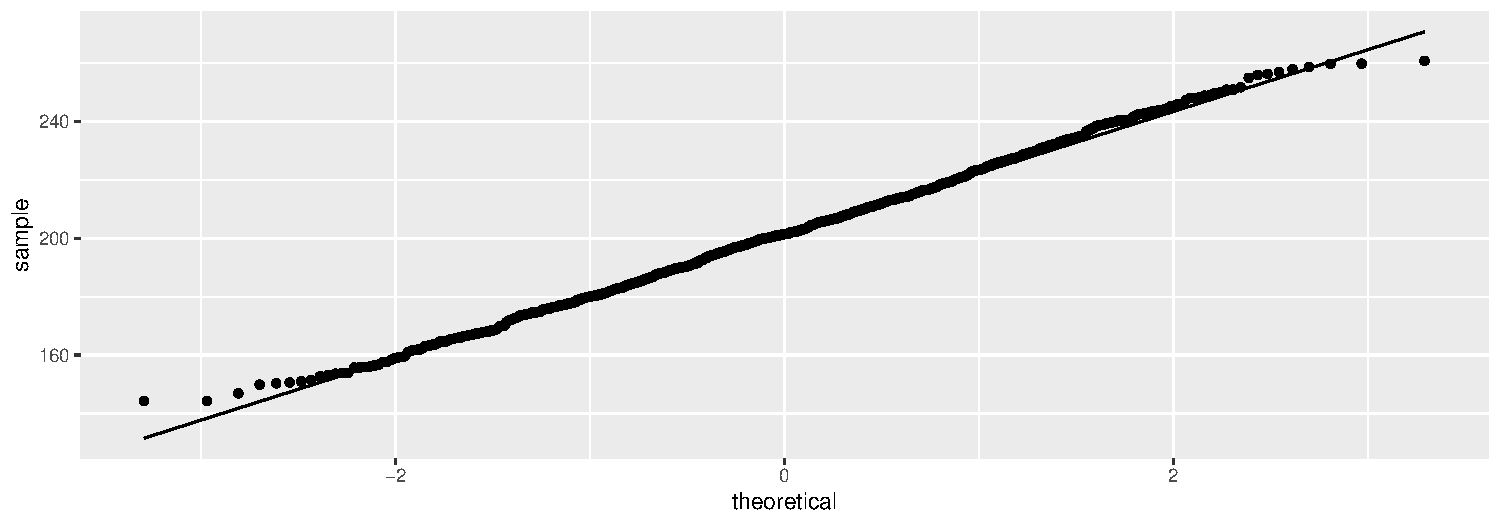
\includegraphics{inference_3_R_slides_files/figure-beamer/unnamed-chunk-11-1.pdf}
\end{frame}

\begin{frame}{Comments}
\protect\hypertarget{comments}{}
\begin{itemize}
\tightlist
\item
  Skewed to right.
\item
  Should look at \emph{median}, not mean.
\end{itemize}
\end{frame}

\begin{frame}{The sign test}
\protect\hypertarget{the-sign-test}{}
\begin{itemize}
\tightlist
\item
  But how to test whether the median is greater than 160?
\item
  Idea: if the median really is 160 (\(H_0\) true), the sampled values
  from the population are equally likely to be above or below 160.
\item
  If the population median is greater than 160, there will be a lot of
  sample values greater than 160, not so many less. Idea: test statistic
  is number of sample values greater than hypothesized median.
\end{itemize}
\end{frame}

\begin{frame}{Getting a P-value for sign test 1/3}
\protect\hypertarget{getting-a-p-value-for-sign-test-13}{}
\begin{itemize}
\tightlist
\item
  How to decide whether ``unusually many'' sample values are greater
  than 160? Need a sampling distribution.
\item
  If \(H_0\) true, pop. median is 160, then each sample value
  independently equally likely to be above or below 160.
\item
  So number of observed values above 160 has binomial distribution with
  \(n = 30\) (number of data values) and \(p = 0.5\) (160 is
  hypothesized to be \emph{median}).
\end{itemize}
\end{frame}

\begin{frame}[fragile]{Getting P-value for sign test 2/3}
\protect\hypertarget{getting-p-value-for-sign-test-23}{}
\begin{itemize}
\tightlist
\item
  Count values above/below 160:
\end{itemize}

\begin{Shaded}
\begin{Highlighting}[]
\NormalTok{irs }\OperatorTok{\%\textgreater{}\%}\StringTok{ }\KeywordTok{count}\NormalTok{(Time }\OperatorTok{\textgreater{}}\StringTok{ }\DecValTok{160}\NormalTok{)}
\end{Highlighting}
\end{Shaded}

\begin{longtable}[]{@{}lr@{}}
\toprule
Time \textgreater{} 160 & n\tabularnewline
\midrule
\endhead
FALSE & 13\tabularnewline
TRUE & 17\tabularnewline
\bottomrule
\end{longtable}

\begin{itemize}
\tightlist
\item
  17 above, 13 below. How unusual is that? Need a \emph{binomial table}.
\end{itemize}
\end{frame}

\begin{frame}[fragile]{Getting P-value for sign test 3/3}
\protect\hypertarget{getting-p-value-for-sign-test-33}{}
\begin{itemize}
\tightlist
\item
  R function \texttt{dbinom} gives the probability of eg. exactly 17
  successes in a binomial with \(n = 30\) and \(p = 0.5\):
\end{itemize}

\begin{Shaded}
\begin{Highlighting}[]
\KeywordTok{dbinom}\NormalTok{(}\DecValTok{17}\NormalTok{, }\DecValTok{30}\NormalTok{, }\FloatTok{0.5}\NormalTok{)}
\end{Highlighting}
\end{Shaded}

\begin{verbatim}
## [1] 0.1115351
\end{verbatim}

\begin{itemize}
\tightlist
\item
  but we want probability of 17 \emph{or more}, so get all of those,
  find probability of each, and add them up:
\end{itemize}

\begin{Shaded}
\begin{Highlighting}[]
\KeywordTok{tibble}\NormalTok{(}\DataTypeTok{x=}\DecValTok{17}\OperatorTok{:}\DecValTok{30}\NormalTok{) }\OperatorTok{\%\textgreater{}\%}\StringTok{ }
\StringTok{  }\KeywordTok{mutate}\NormalTok{(}\DataTypeTok{prob=}\KeywordTok{dbinom}\NormalTok{(x, }\DecValTok{30}\NormalTok{, }\FloatTok{0.5}\NormalTok{)) }\OperatorTok{\%\textgreater{}\%}\StringTok{ }
\StringTok{  }\KeywordTok{summarize}\NormalTok{(}\DataTypeTok{total=}\KeywordTok{sum}\NormalTok{(prob))}
\end{Highlighting}
\end{Shaded}

\begin{longtable}[]{@{}r@{}}
\toprule
total\tabularnewline
\midrule
\endhead
0.2923324\tabularnewline
\bottomrule
\end{longtable}
\end{frame}

\begin{frame}[fragile]{Using my package \texttt{smmr}}
\protect\hypertarget{using-my-package-smmr}{}
\begin{itemize}
\tightlist
\item
  I wrote a package \texttt{smmr} to do the sign test (and some other
  things). Installation is a bit fiddly:

  \begin{itemize}
  \tightlist
  \item
    Install devtools with \texttt{install.packages("devtools")}
  \item
    then install smmr:
  \end{itemize}
\end{itemize}

\begin{Shaded}
\begin{Highlighting}[]
\KeywordTok{library}\NormalTok{(devtools)}
\KeywordTok{install\_github}\NormalTok{(}\StringTok{"nxskok/smmr"}\NormalTok{)}
\end{Highlighting}
\end{Shaded}

\begin{itemize}
\tightlist
\item
  Then load it:
\end{itemize}

\begin{Shaded}
\begin{Highlighting}[]
\KeywordTok{library}\NormalTok{(smmr)}
\end{Highlighting}
\end{Shaded}
\end{frame}

\begin{frame}[fragile]{\texttt{smmr} for sign test}
\protect\hypertarget{smmr-for-sign-test}{}
\begin{itemize}
\tightlist
\item
  \texttt{smmr}'s function \texttt{sign\_test} needs three inputs: a
  data frame, a column and a null median:
\end{itemize}

\begin{Shaded}
\begin{Highlighting}[]
\KeywordTok{sign\_test}\NormalTok{(irs, Time, }\DecValTok{160}\NormalTok{)}
\end{Highlighting}
\end{Shaded}

\begin{verbatim}
## $above_below
## below above 
##    13    17 
## 
## $p_values
##   alternative   p_value
## 1       lower 0.8192027
## 2       upper 0.2923324
## 3   two-sided 0.5846647
\end{verbatim}
\end{frame}

\begin{frame}{Comments (1/3)}
\protect\hypertarget{comments-13}{}
\begin{itemize}
\tightlist
\item
  Testing whether population median \emph{greater than} 160, so want
  \emph{upper-tail} P-value 0.2923. Same as before.
\item
  Also get table of values above and below; this too as we got.
\end{itemize}
\end{frame}

\begin{frame}[fragile]{Comments (2/3)}
\protect\hypertarget{comments-23}{}
\begin{itemize}
\tightlist
\item
  P-values are:

  \begin{center}
    \begin{tabular}{lr}
      Test & P-value\\
      \hline
      $t$ & 0.0392\\
      Sign & 0.2923\\
      \hline
    \end{tabular}

    \end{center}
\item
  These are very different: we reject a mean of 160 (in favour of the
  mean being bigger), but clearly \emph{fail} to reject a median of 160
  in favour of a bigger one.
\item
  Why is that? Obtain mean and median:
\end{itemize}

\begin{Shaded}
\begin{Highlighting}[]
\NormalTok{irs }\OperatorTok{\%\textgreater{}\%}\StringTok{ }\KeywordTok{summarize}\NormalTok{(}\DataTypeTok{mean\_time =} \KeywordTok{mean}\NormalTok{(Time), }
                  \DataTypeTok{median\_time =} \KeywordTok{median}\NormalTok{(Time))}
\end{Highlighting}
\end{Shaded}

\begin{longtable}[]{@{}rr@{}}
\toprule
mean\_time & median\_time\tabularnewline
\midrule
\endhead
201.2333 & 172.5\tabularnewline
\bottomrule
\end{longtable}
\end{frame}

\begin{frame}{Comments (3/3)}
\protect\hypertarget{comments-33}{}
\begin{itemize}
\tightlist
\item
  The mean is pulled a long way up by the right skew, and is a fair bit
  bigger than 160.
\item
  The median is quite close to 160.
\item
  We ought to be trusting the sign test and not the t-test here (median
  and not mean), and therefore there is no evidence that the ``typical''
  time to complete the form is longer than 160 minutes.
\item
  Having said that, there are clearly some people who take a lot longer
  than 160 minutes to complete the form, and the IRS could focus on
  simplifying its form for these people.
\item
  In this example, looking at any kind of average is not really helpful;
  a better question might be ``do an unacceptably large fraction of
  people take longer than (say) 300 minutes to complete the form?'':
  that is, thinking about worst-case rather than average-case.
\end{itemize}
\end{frame}

\begin{frame}{Confidence interval for the median}
\protect\hypertarget{confidence-interval-for-the-median}{}
\begin{itemize}
\tightlist
\item
  The sign test does not naturally come with a confidence interval for
  the median.
\item
  So we use the ``duality'' between test and confidence interval to say:
  the (95\%) confidence interval for the median contains exactly those
  values of the null median that would not be rejected by the two-sided
  sign test (at \(\alpha = 0.05\)).
\end{itemize}
\end{frame}

\begin{frame}[fragile]{For our data}
\protect\hypertarget{for-our-data}{}
\begin{itemize}
\tightlist
\item
  The procedure is to try some values for the null median and see which
  ones are inside and which outside our CI.
\item
  smmr has pval\_sign that gets just the 2-sided P-value:
\end{itemize}

\begin{Shaded}
\begin{Highlighting}[]
\KeywordTok{pval\_sign}\NormalTok{(}\DecValTok{160}\NormalTok{, irs, Time)}
\end{Highlighting}
\end{Shaded}

\begin{verbatim}
## [1] 0.5846647
\end{verbatim}

\begin{itemize}
\tightlist
\item
  Try a couple of null medians:
\end{itemize}

\begin{Shaded}
\begin{Highlighting}[]
\KeywordTok{pval\_sign}\NormalTok{(}\DecValTok{200}\NormalTok{, irs, Time)}
\end{Highlighting}
\end{Shaded}

\begin{verbatim}
## [1] 0.3615946
\end{verbatim}

\begin{Shaded}
\begin{Highlighting}[]
\KeywordTok{pval\_sign}\NormalTok{(}\DecValTok{300}\NormalTok{, irs, Time)}
\end{Highlighting}
\end{Shaded}

\begin{verbatim}
## [1] 0.001430906
\end{verbatim}

\begin{itemize}
\tightlist
\item
  So 200 inside the 95\% CI and 300 outside.
\end{itemize}
\end{frame}

\begin{frame}[fragile]{Doing a whole bunch}
\protect\hypertarget{doing-a-whole-bunch}{}
\begin{itemize}
\tightlist
\item
  Choose our null medians first:
\end{itemize}

\small

\begin{Shaded}
\begin{Highlighting}[]
\NormalTok{(}\DataTypeTok{d=}\KeywordTok{tibble}\NormalTok{(}\DataTypeTok{null\_median=}\KeywordTok{seq}\NormalTok{(}\DecValTok{100}\NormalTok{,}\DecValTok{300}\NormalTok{,}\DecValTok{20}\NormalTok{)))}
\end{Highlighting}
\end{Shaded}

\begin{longtable}[]{@{}r@{}}
\toprule
null\_median\tabularnewline
\midrule
\endhead
100\tabularnewline
120\tabularnewline
140\tabularnewline
160\tabularnewline
180\tabularnewline
200\tabularnewline
220\tabularnewline
240\tabularnewline
260\tabularnewline
280\tabularnewline
300\tabularnewline
\bottomrule
\end{longtable}

\normalsize
\end{frame}

\begin{frame}[fragile]{\ldots{} and then}
\protect\hypertarget{and-then}{}
``for each null median, run the function \texttt{pval\_sign} for that
null median and get the P-value'':

\begin{Shaded}
\begin{Highlighting}[]
\NormalTok{d }\OperatorTok{\%\textgreater{}\%}\StringTok{ }\KeywordTok{mutate}\NormalTok{(}\DataTypeTok{p\_value =} \KeywordTok{map\_dbl}\NormalTok{(null\_median, }
                               \OperatorTok{\textasciitilde{}}\StringTok{ }\KeywordTok{pval\_sign}\NormalTok{(., irs, Time)))}
\end{Highlighting}
\end{Shaded}

\begin{longtable}[]{@{}rr@{}}
\toprule
null\_median & p\_value\tabularnewline
\midrule
\endhead
100 & 0.0003249\tabularnewline
120 & 0.0987371\tabularnewline
140 & 0.2004884\tabularnewline
160 & 0.5846647\tabularnewline
180 & 0.8555356\tabularnewline
200 & 0.3615946\tabularnewline
220 & 0.0427739\tabularnewline
240 & 0.0161248\tabularnewline
260 & 0.0052229\tabularnewline
280 & 0.0014309\tabularnewline
300 & 0.0014309\tabularnewline
\bottomrule
\end{longtable}
\end{frame}

\begin{frame}[fragile]{Make it easier for ourselves}
\protect\hypertarget{make-it-easier-for-ourselves}{}
\begin{Shaded}
\begin{Highlighting}[]
\NormalTok{d }\OperatorTok{\%\textgreater{}\%}\StringTok{ }
\StringTok{  }\KeywordTok{mutate}\NormalTok{(}\DataTypeTok{p\_value =} \KeywordTok{map\_dbl}\NormalTok{(null\_median, }
                           \OperatorTok{\textasciitilde{}}\StringTok{ }\KeywordTok{pval\_sign}\NormalTok{(., irs, Time))) }\OperatorTok{\%\textgreater{}\%}
\StringTok{  }\KeywordTok{mutate}\NormalTok{(}\DataTypeTok{in\_out =} \KeywordTok{ifelse}\NormalTok{(p\_value }\OperatorTok{\textgreater{}}\StringTok{ }\FloatTok{0.05}\NormalTok{, }\StringTok{"inside"}\NormalTok{, }\StringTok{"outside"}\NormalTok{))}
\end{Highlighting}
\end{Shaded}

\begin{longtable}[]{@{}rrl@{}}
\toprule
null\_median & p\_value & in\_out\tabularnewline
\midrule
\endhead
100 & 0.0003249 & outside\tabularnewline
120 & 0.0987371 & inside\tabularnewline
140 & 0.2004884 & inside\tabularnewline
160 & 0.5846647 & inside\tabularnewline
180 & 0.8555356 & inside\tabularnewline
200 & 0.3615946 & inside\tabularnewline
220 & 0.0427739 & outside\tabularnewline
240 & 0.0161248 & outside\tabularnewline
260 & 0.0052229 & outside\tabularnewline
280 & 0.0014309 & outside\tabularnewline
300 & 0.0014309 & outside\tabularnewline
\bottomrule
\end{longtable}
\end{frame}

\begin{frame}{confidence interval for median?}
\protect\hypertarget{confidence-interval-for-median}{}
\begin{itemize}
\tightlist
\item
  95\% CI to this accuracy from 120 to 200.
\item
  Can get it more accurately by looking more closely in intervals from
  100 to 120, and from 200 to 220.
\end{itemize}
\end{frame}

\begin{frame}[fragile]{A more efficient way: bisection}
\protect\hypertarget{a-more-efficient-way-bisection}{}
\begin{itemize}
\tightlist
\item
  Know that top end of CI between 200 and 220:
\end{itemize}

\begin{Shaded}
\begin{Highlighting}[]
\NormalTok{lo=}\DecValTok{200} 
\NormalTok{hi=}\DecValTok{220}
\end{Highlighting}
\end{Shaded}

\begin{itemize}
\tightlist
\item
  Try the value halfway between: is it inside or outside?
\end{itemize}

\begin{Shaded}
\begin{Highlighting}[]
\NormalTok{(}\DataTypeTok{try =}\NormalTok{ (lo }\OperatorTok{+}\StringTok{ }\NormalTok{hi) }\OperatorTok{/}\StringTok{ }\DecValTok{2}\NormalTok{)}
\end{Highlighting}
\end{Shaded}

\begin{verbatim}
## [1] 210
\end{verbatim}

\begin{Shaded}
\begin{Highlighting}[]
\KeywordTok{pval\_sign}\NormalTok{(try,irs,Time)}
\end{Highlighting}
\end{Shaded}

\begin{verbatim}
## [1] 0.09873715
\end{verbatim}

\begin{itemize}
\tightlist
\item
  Inside, so upper end is between 210 and 220. Repeat (over):
\end{itemize}
\end{frame}

\begin{frame}[fragile]{\ldots{} bisection continued}
\protect\hypertarget{bisection-continued}{}
\begin{Shaded}
\begin{Highlighting}[]
\NormalTok{lo =}\StringTok{ }\NormalTok{try}
\NormalTok{(}\DataTypeTok{try =}\NormalTok{ (lo }\OperatorTok{+}\StringTok{ }\NormalTok{hi) }\OperatorTok{/}\StringTok{ }\DecValTok{2}\NormalTok{)}
\end{Highlighting}
\end{Shaded}

\begin{verbatim}
## [1] 215
\end{verbatim}

\begin{Shaded}
\begin{Highlighting}[]
\KeywordTok{pval\_sign}\NormalTok{(try, irs, Time)}
\end{Highlighting}
\end{Shaded}

\begin{verbatim}
## [1] 0.06142835
\end{verbatim}

\begin{itemize}
\tightlist
\item
  215 is inside too, so upper end between 215 and 220.
\item
  Continue until have as accurate a result as you want.
\end{itemize}
\end{frame}

\begin{frame}[fragile]{Bisection automatically}
\protect\hypertarget{bisection-automatically}{}
\begin{itemize}
\tightlist
\item
  A loop, but not a \texttt{for} since we don't know how many times
  we're going around. Keep going while a condition is true:
\end{itemize}

\begin{Shaded}
\begin{Highlighting}[]
\NormalTok{lo =}\StringTok{ }\DecValTok{200}
\NormalTok{hi =}\StringTok{ }\DecValTok{220}
\ControlFlowTok{while}\NormalTok{ (hi }\OperatorTok{{-}}\StringTok{ }\NormalTok{lo }\OperatorTok{\textgreater{}}\StringTok{ }\DecValTok{1}\NormalTok{) \{}
\NormalTok{  try =}\StringTok{ }\NormalTok{(hi }\OperatorTok{+}\StringTok{ }\NormalTok{lo) }\OperatorTok{/}\StringTok{ }\DecValTok{2}
\NormalTok{  ptry =}\StringTok{ }\KeywordTok{pval\_sign}\NormalTok{(try, irs, Time)}
  \KeywordTok{print}\NormalTok{(}\KeywordTok{c}\NormalTok{(try, ptry))}
  \ControlFlowTok{if}\NormalTok{ (ptry }\OperatorTok{\textless{}=}\StringTok{ }\FloatTok{0.05}\NormalTok{)}
\NormalTok{    hi =}\StringTok{ }\NormalTok{try}
  \ControlFlowTok{else}
\NormalTok{    lo =}\StringTok{ }\NormalTok{try}
\NormalTok{\}}
\end{Highlighting}
\end{Shaded}
\end{frame}

\begin{frame}[fragile]{The output from this loop}
\protect\hypertarget{the-output-from-this-loop}{}
\begin{verbatim}
## [1] 210.00000000   0.09873715
## [1] 215.00000000   0.06142835
## [1] 217.50000000   0.04277395
## [1] 216.25000000   0.04277395
## [1] 215.62500000   0.04277395
\end{verbatim}

\begin{itemize}
\tightlist
\item
  215 inside, 215.625 outside. Upper end of interval to this accuracy is
  215.
\end{itemize}
\end{frame}

\begin{frame}[fragile]{Using smmr}
\protect\hypertarget{using-smmr}{}
\begin{itemize}
\tightlist
\item
  \texttt{smmr} has function \texttt{ci\_median} that does this (by
  default 95\% CI):
\end{itemize}

\begin{Shaded}
\begin{Highlighting}[]
\KeywordTok{ci\_median}\NormalTok{(irs,Time)}
\end{Highlighting}
\end{Shaded}

\begin{verbatim}
## [1] 119.0065 214.9955
\end{verbatim}

\begin{itemize}
\tightlist
\item
  Uses a more accurate bisection than we did.
\item
  Or get, say, 90\% CI for median:
\end{itemize}

\begin{Shaded}
\begin{Highlighting}[]
\KeywordTok{ci\_median}\NormalTok{(irs,Time,}\DataTypeTok{conf.level=}\FloatTok{0.90}\NormalTok{)}
\end{Highlighting}
\end{Shaded}

\begin{verbatim}
## [1] 123.0031 208.9960
\end{verbatim}

\begin{itemize}
\tightlist
\item
  90\% CI is shorter, as it should be.
\end{itemize}
\end{frame}

\begin{frame}[fragile]{Bootstrap (optional)}
\protect\hypertarget{bootstrap-optional}{}
\begin{itemize}
\tightlist
\item
  but, was the sample size (30) big enough to overcome the skewness?
\item
  Bootstrap, again:
\end{itemize}

\begin{Shaded}
\begin{Highlighting}[]
\KeywordTok{rerun}\NormalTok{(}\DecValTok{1000}\NormalTok{, }\KeywordTok{sample}\NormalTok{(irs}\OperatorTok{$}\NormalTok{Time, }\DataTypeTok{replace =} \OtherTok{TRUE}\NormalTok{)) }\OperatorTok{\%\textgreater{}\%}\StringTok{ }
\StringTok{  }\KeywordTok{map\_dbl}\NormalTok{(}\OperatorTok{\textasciitilde{}}\KeywordTok{mean}\NormalTok{(.)) }\OperatorTok{\%\textgreater{}\%}\StringTok{ }
\StringTok{  }\KeywordTok{enframe}\NormalTok{() }\OperatorTok{\%\textgreater{}\%}\StringTok{ }
\StringTok{  }\KeywordTok{ggplot}\NormalTok{(}\KeywordTok{aes}\NormalTok{(}\DataTypeTok{x=}\NormalTok{value)) }\OperatorTok{+}\StringTok{ }\KeywordTok{geom\_histogram}\NormalTok{(}\DataTypeTok{bins=}\DecValTok{10}\NormalTok{) {-}\textgreater{}}\StringTok{ }\NormalTok{g}
\end{Highlighting}
\end{Shaded}
\end{frame}

\begin{frame}[fragile]{The sampling distribution}
\protect\hypertarget{the-sampling-distribution}{}
\begin{Shaded}
\begin{Highlighting}[]
\NormalTok{g}
\end{Highlighting}
\end{Shaded}

\includegraphics{inference_3_R_slides_files/figure-beamer/unnamed-chunk-33-1.pdf}
\end{frame}

\begin{frame}{Comments}
\protect\hypertarget{comments-1}{}
\begin{itemize}
\tightlist
\item
  A little skewed to right, but not nearly as much as I was expecting.
\item
  The \(t\)-test for the mean might actually be OK for these data,
  \emph{if the mean is what you want}.
\item
  In actual data, mean and median very different; we chose to make
  inference about the median.
\item
  Thus for us it was right to use the sign test.
\end{itemize}
\end{frame}

\end{document}
